% vim: set fecn=utf8 ft=latex encoding=utf8
% -*- mode: latex; coding: UTF-8; -*-

\newif\ifdraft
% \drafttrue

%%% blobtree.tex

\ifdraft
	\documentclass[conference]{acmsiggraph}
	\def\baselinestrech{1}
	\setlength{\marginparwidth}{2cm}
	\newcommand{\Title}{Implementing the Blob Tree | Draft}
\else
	\documentclass[conference]{acmsiggraph}
	\newcommand{\Title}{Implementing the Blob Tree}
\fi

\newcommand{\Author}{Evan T. C. Wilde}
\newcommand{\Email}{etcwilde@uvic.ca}
\newcommand{\Subject}{Implementing the Blob Tree}
\newcommand{\Keywords}{implicit surface, iso-surface, blobs, blobbies, blobtree}

\synctex=1

\usepackage{longtable}
\usepackage{multirow}

\usepackage{xspace}
\usepackage{amssymb}
\usepackage{amsmath}
\usepackage{breqn}
\usepackage{svg}

\ifdraft
	\hypersetup{pdftitle={\Title},
		pdfauthor={\Author},
		pdfkeywords={\Keywords},
		pdfsubject={\Subject},
		urlcolor=blue,citecolor=red}
\else
	\hypersetup{pdftitle={\Title},
		pdfauthor={\Author},
		pdfkeywords={\Keywords},
		pdfsubject={\Subject},
		urlcolor=black,citecolor=black}
\fi

\def\BibTeX{{\rm B\kern-.05em{\sc i\kern-.025em b}\kern-.08em
    T\kern-.1667em\lower.7ex\hbox{E}\kern-.125emX}}

\TOGonlineid{000000000}
\TOGvolume{0}
\TOGnumber{0}

\ifdraft
	\usepackage[colorinlistoftodos]{todonotes}
		\newcommand{\evan}[1]{{\color{cyan}\emph{Evan Says:
		#1}}\xspace}
		\newcommand{\evanTodo}[1]{{\color{blue}\emph{Evan Todo:
		#1}}\xspace}
\else
	\usepackage[disable]{todonotes}
	\newcommand{\evan}[1]{}
	\newcommand{\evanTodo}[1]{}
\fi

\newcommand{\fff}{field falloff function}


%%% Local Variables:
%%% mode: latex
%%% TeX-master: "marching-triangles"
%%% End:


\title{\Title}
\author{
	\Author \\
	University of Victoria\\
\Email}
\pdfauthor{\Author}
\keywords{\Keywords}

\begin{document}

\teaser{
	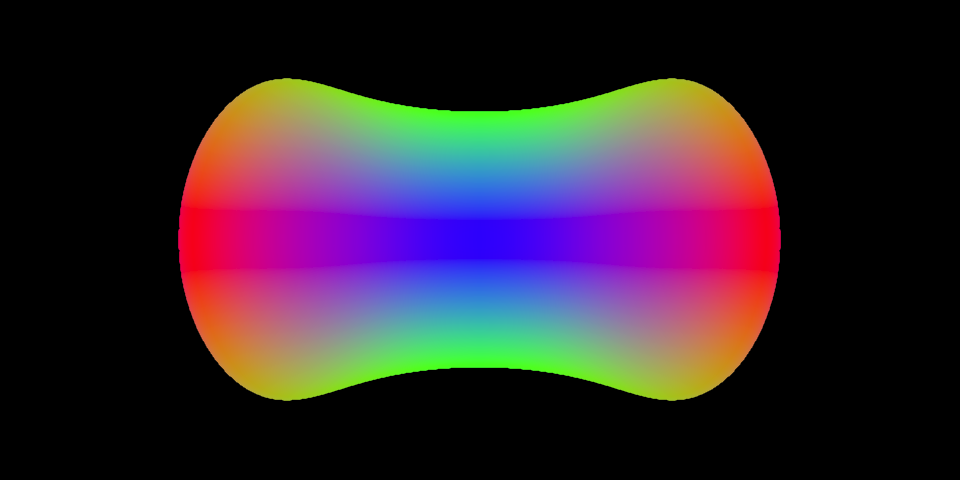
\includegraphics[height=1.5in] {images/blend.png}
	\caption{Blended Blobs}
}

\maketitle

\begin{abstract}
	Implicit surfaces are a mathematical representation of geometric
	information; storing complex geometric information with minimal memory
	requirements.

	A form of implicit surface uses the algebraic form of the
	shape, for example a sphere is represented by the equation $x^2 + y^2 +
	z^2 = R^2$. These equations become complex very quickly as the geometry
	becomes more complicated, so the CSG was developed to allow the
	construction of complex geometry from simpler primitive objects.

	Blobs are a different form of implicit object, defined by a central
	origin point, a field falloff function, and an iso value. The surface
	itself is then defined at the distance from the origin point where the
	field falloff function evaluates to the iso value. Blobs were used for
	modeling electron density fields in the 80's due to their ability to
	blend together and to effect the shape of other nearby blobs. Since
	then their use has grown to encompass other geometries. A blob tree is
	to blobs as a CSG is to the algebraic form of implicit surfaces. It
	permits the construction of complex geometries through the use of
	union, intersect and difference operations, with the additional bonus
	of the blend operation.

	Since blobs can interact with each other, some of the optimizations made
	on CSGs are not available, making intelligent construction of the blob
	tree critical for fast evaluation of the implicit object represented
	in the tree, whether the evaluation is for ray-tracing or
	polygonization.

	In this paper, we explore the implementation details of a simple blob
	tree and look into various techniques for getting better performance
	and more robustness from our blob tree.

\end{abstract}

\keywordlist

\copyrightspace

\section{Introduction}

Implicit surfaces are a mathematical representation of geometric information;
storing complex geometric information with minimal memory requirements.
Implicit surfaces can be represented with implicit equations or as blobs. The
implicit equation form uses algebraic formulas to define shapes, for example a
sphere is represented by the equations $x^2 + y^2 + z^2 = R^2$, where $R$ is
the radius of the sphere. A more complex shape defined by an implicit equation
is a jack,

\begin{dmath*}
\left({1 \over ({x^2 \over 9} +  4y^2 + 4z^2)^4} +
{1 \over ({y^2 \over 9} +  4x^2 + 4z^2)^4} +
{1 \over (({4x \over 3} - 4)^2 + {16y^2 \over 9} +  {16z^2 \over 9})^4} +
{1 \over (({4x \over 3} + 4)^2 + {16y^2 \over 9} +  {16z^2 \over 9})^4} +
{1 \over (({4y \over 3} - 4)^2 + {16x^2 \over 9} +  {16z^2 \over 9})^4} +
{1 \over (({4y \over 3} + 4)^2 + {16x^2 \over 9} +  {16z^2 \over 9})^4}\right)^ {-
	{1\over 4}} - 1
\end{dmath*}
\cite{Bloomenthal1994}

Due to the complexity of the algebraic equations for complex models, a new model
was proposed which constructed complex geometry from simpler primitives using
the operations union, different, and intersect. This model was called CSG, or
constructive solid geometry.

A separate form of the implicit surface is the blob, or blobby molecule,
defined by Jim Blinn\cite{Blinn} for observing the behaviour of electron
density fields. Blobs are defined in three parts: a center point, a
field falloff function, and an iso value. The central point is the point around
which the blob surface exists. 
The field falloff function is a function where at
the center point is at its highest value, and at some maximum radius $R$
evaluates to 0. The surface itself is then defined at the distance $r$ from the
origin point where the field falloff function evaluates to the iso value.

Brian Wyvill proposed a new structure combining the power of CSG trees and
blobs into one structure, the blob tree. Blob trees are a data structure for
containing and evaluating geometric information stored as blobs. A blob tree
represents the complex geometry in a hierarchy where the root node is the
intended shape and the leaf nodes are the primitive objects. The interior nodes
are the various operations that can be performed on the primitives and simpler
objects. These operations can be combined in various ways to design more
complex objects.

In this paper, we explore the implementation details of a simple blob tree
structure and the various additions that can be implemented to increase the
performance and robustness of the tree for various uses.

The implementation of the tree is available on
GitHub\footnote{\url{https://github.com/etcwilde/ImplicitSystem}}, with the
accommodating implementation of the raytracer used to generate the images
within this papers\footnote{\url{https://github.com/etcwilde/ImplictRaytacer}}.

\section{Related Work}
Jim Blinn used blobs, or blobby molecules as a way of representing electron
density fields\cite{Blinn}. Using blobs as a way of modeling has interesting
advantages to simply working with algebraic implicit surfaces. Brian Wyvill
worked to combine the power of CSG trees and blending of blobs to create a new
implicit system, the blob tree. Blob trees are capable of all the basic CSG
operations, such as union, intersect, difference, and warp, but also include
the blend operation which will blend the blobs together when they get within a
certain distance of each other. That is, the blobs can effect the shape of the
blobs surrounding it.

\section{Implementation Details}
In this section, we describe the methods of implementing the blob tree, and why
we made a given decision.


\subsection{Finding Surface}
Finding the point where the surface exists proves to be challenging, as the
field falloff function is not necessarily invertible. To find the surface, a numerical
root-finding method is required. I used the secant method, described as
follows:
\begin{equation}
x_i = x_{i-1} - f(x_{i-1}) \times {x_{i-1} - x_{i-2} \over f(x_{i-1}) -
f(x_{i-2})}
\label{eq:SecantMethod}
\end{equation}

The secant method was chosen due to the relative speed of convergence, not
requiring bracketing, and not requiring derivations. The bisection method
guarantees convergence and does not require differentiation; however, it
requires a bracket to be placed around the surface, and has linear convergence. The
Newton-Raphson method is an open method that has order $n^2$ convergence, but
requires derivations and cannot guarantee convergence. The secant method is
another open method that has order $n^{1.618}$ convergence and does not require
derivations, but cannot guarantee convergence. Furthermore, as an open interval
method, the initial point must be close enough to the shape that the \fff\ has
an effect.

For the purpose of polygonization, it is possible to use the centre point of a
given primitive, which will be at the centre of the field function. In most
cases, given the Geoff \fff, the secant method will converge within 6
iterations. For this purpose, no extra measures are necessary to ensure
convergence.

\begin{figure}[htb]
	\centering
	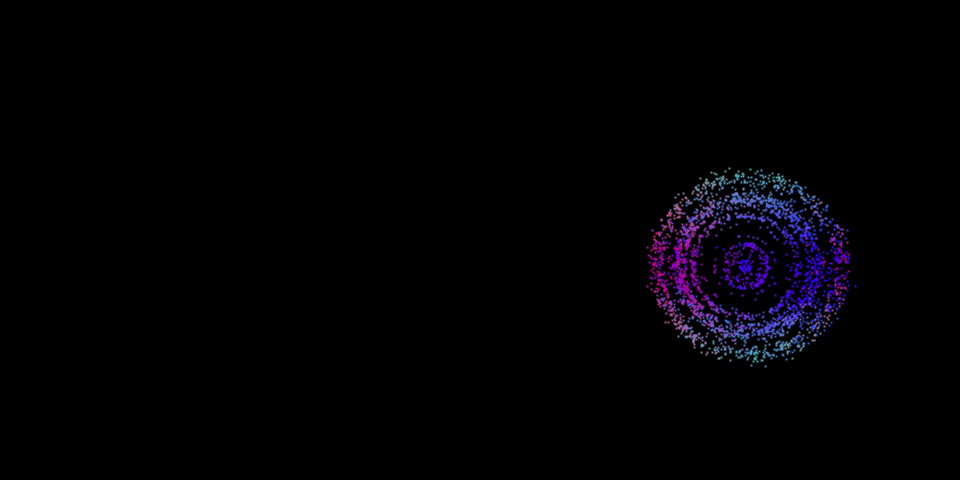
\includegraphics[height=1.5in] {images/sphere_no_bvh.png}
	\caption{Ray-traced blob without bvh}
	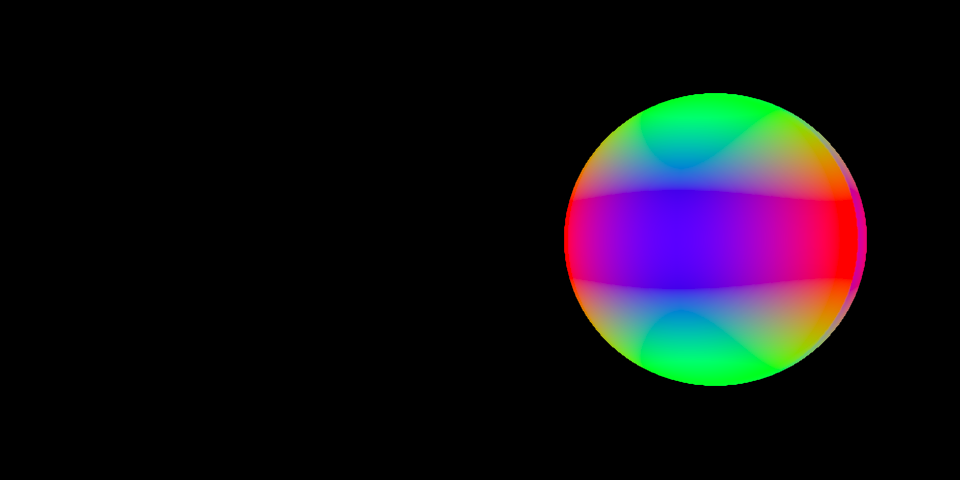
\includegraphics[height=1.5in] {images/sphere_bvh.png}
	\caption{Ray-traced blob with bvh}
\end{figure}

For the purpose of raytracing, in most cases the rays being sent toward the
object are beyond the maximum radius of the \fff\ and the secant method is
unable to converge. For this, we implemented a simple bounding volume
hierarchy, which is able to quickly determine which rays get close enough to
the surface that the \fff\ will have values different than zero.

\subsection{Primitives}
The current implementation has the spherical blob primitive. This is the
simplest primitive for blobs to represent. A spherical blob consists of a
centre point $center$, a field falloff function $f(r)$, and an iso value
$iso$ where the surface is defined.

The field falloff function we have implemented is the Geoff function: $r$ is
the defined by the distance from the central point, $R$ is the maximum
effective distance of the field falloff function.
\begin{equation}
f(r) = 1 - {4\over9} {r^6 \over R^6} + {17 \over 9} {r^4 \over R ^ 4} -
{22\over 9} {r^2 \over R^2}
\label{eq:GeoffFunction}
\end{equation}

In the blob tree, primitive objects are the simplest object and therefore are
always leaf nodes.

\textbf{Evaluating the field function}\\
Given $p$ and a sphere primitive, the field value is evaluated as:

\begin{equation}
F(p) = f(\lvert p - center \rvert)\\
\label{eq:FieldValue}
\end{equation}
\begin{equation}
E(p) = f(\lvert p - center \rvert) - iso
\label{eq:SurfaceEvaluate}
\end{equation}



In equation (\ref{eq:FieldValue}), the result of the function must be compared with
the iso value to determine where the surface is. For this reason, it is helpful
to simply define another function (\ref{eq:SurfaceEvaluate}) which subtracts the
iso value from the evalutated field value. To distinguish the two functions I
call function (\ref{eq:FieldValue}) ``Field evaluation'', and function
(\ref{eq:SurfaceEvaluate}) ``Surface evaluation''.

Equation  (\ref{eq:FieldValue}) is called during the traversal of the tree. This
is useful for performing the various operations on the primitive objects.
Equation (\ref{eq:SurfaceEvaluate}) is used primarily for the purpose of root
finding, since the root-finding method will tend to zero rather than an
arbitrary value. Furthermore, the surface evaluation function
(\ref{eq:SurfaceEvaluate}) behaves more like the algebraic form of implicit
surfaces over the blob-form of implicit surfaces.


\textbf{Evaluating the normal}\\
Given $p$ and a sphere primitive, the normal is evaluated as:
$$ \overrightarrow{N}(p) = {p - center \over \lvert p - center \rvert}$$

\subsection{Transforms}
We implemented the three basic transforms: translation, rotation, and scaling.
The transform class simply takes any 3-dimensional homogeneous matrix, making
the implementation of the translation, rotation, and scaling operations
trivial. The use of an over-arching transform class simplifies the
implementation.

\begin{figure}[htb]
	\centering
	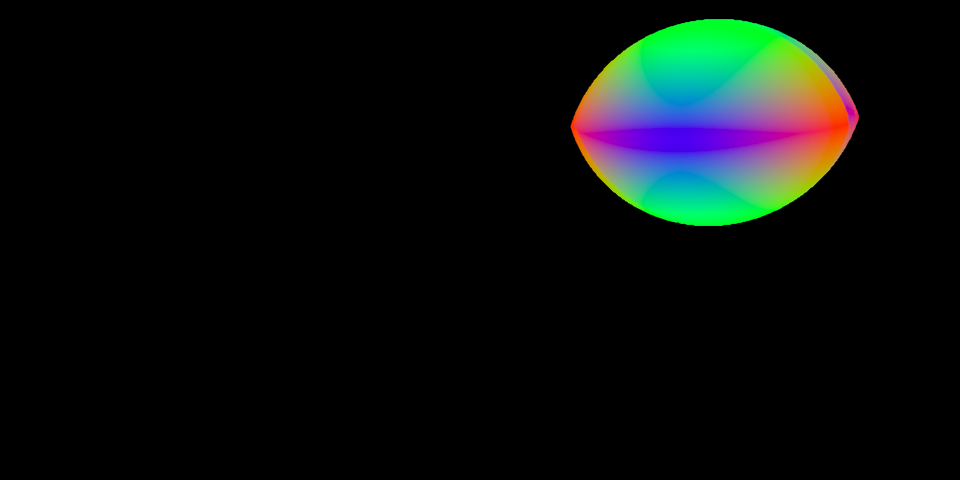
\includegraphics[height=1.5in]{images/intersect_rotate.png}
	\caption{Intersected Spheres Rotated then Translated}
\end{figure}

For shape-preserving transformation, no additional work is necessary for
calculating normal vectors. Shape-preserving transformations include
translation and rotation, a transform that does not preserve the shape is the
skew operation. To find the normal of a shape-preserving transform, we map the
test point to the local coordinates, and return the normal from the child
object at the point in local coordinates. If the transform is not
shape-preserving, we must calculate the inverse transpose matrix from the
transform matrix, and multiply the normal vector with that matrix.

\subsection{Operations}
Blob-trees are able to perform various binary operations between two
sub-trees. Our implementation provides three of the five possible operations;
the blend, union, and intersect operations. The two remaining operations are
the warp, which is not a binary operation, but includes tapers and twisting,
and difference, allowing blobs to remove volume from another blob.

In section \ref{subsec:Tree Traversal} we describe the implementation of the
field evaluation, surface evaluation, and normal calculation for all
operations.The method for calculating the field values of the various
operations is further described in \textit{The BlobTree} \cite{Wyvill}.

\subsubsection{Blend}
\begin{figure}[htbp]
	\centering
	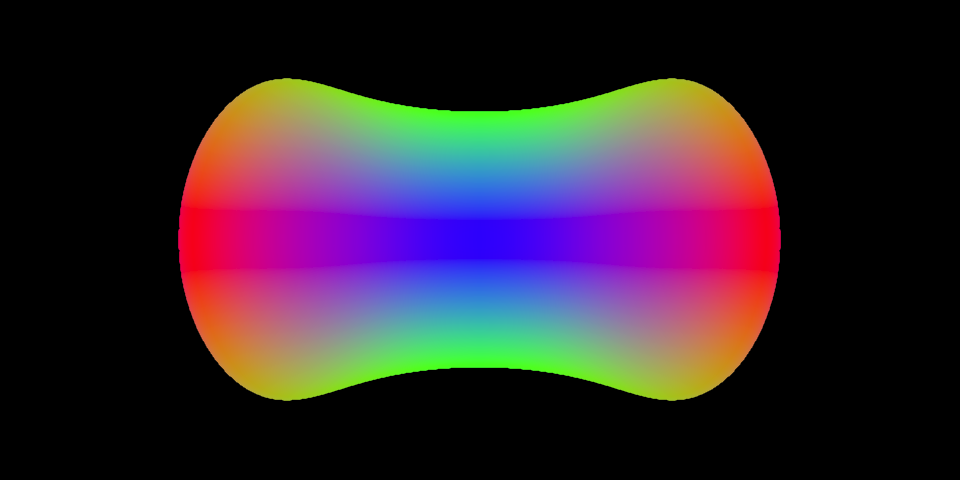
\includegraphics[height=1.5in]{images/blend.png}
	\caption{Blend operation}
	\label{fig:Blend}
\end{figure}

The blend operation is what gives blobs more functionality than the algebraic
form of implicit surface. The blended field value is defined by adding the
field values of the component objects together at a desired point. We see the
effects of the blend operation in figure \ref{fig:Blend}. It is due to the
effect of the field falloff function summing together that we can get this
extra operation at no extra cost. The cost is built into the blob model.

\subsubsection{Union}
\begin{figure}[htbp]
	\centering
	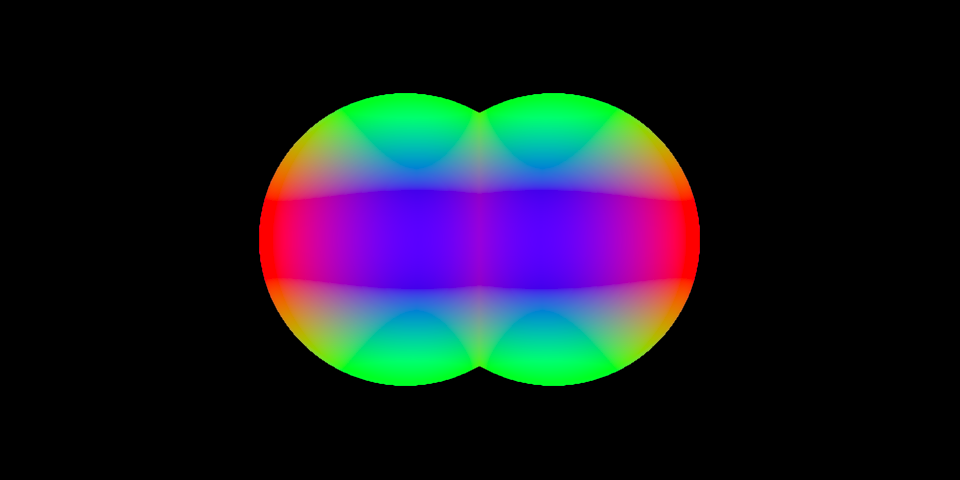
\includegraphics[height=1.5in]{images/union.png}
	\caption{Union operation}
	\label{fig:Union}
\end{figure}

The union simply unions the two simpler objects into a single more complex
object. No blending or warping should occur to either child shape. A sharp edge
may occur of the two objects being unioned are touching. The valley formed
where they touch is a sharp edge and loses curvature and normal information,
as shown in figure \ref{fig:UnionSharpEdge}. The union is found by taking the
maximum field values of both child objects.


\subsubsection{Intersect}
\begin{figure}[htbp]
	\centering
	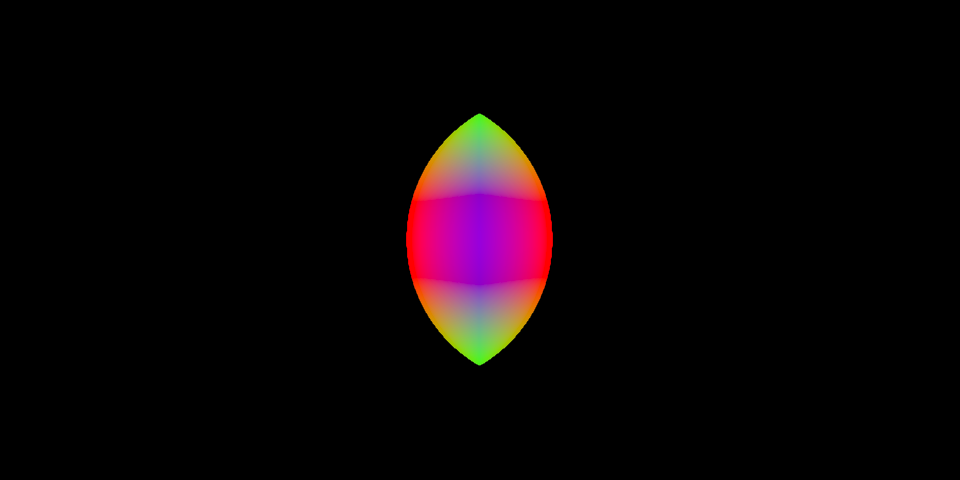
\includegraphics[height=1.5in]{images/intersect.png}
	\caption{Intersect operation}
	\label{fig:Intersection}
\end{figure}

The intersection operations leaves geometry where the two objects overlap. A
sharp edge may occur as shown in \ref{fig:IntersectSharpEdge}. The intersection
is found by taking the minimum of the field values





\subsection{Tree Traversal\label{subsec:Tree Traversal}}
In this section, we describe how to traverse the tree, evaluating the field
value, the surface value, and the normal.

We will use notation similar to the object-oriented paradigm. For a given
object $O$, we will use $O.center$ to represent the center of the object,
$O.iso$ to represent the iso value of the object, and $O.f(r)$ to represent the
field function of the object.

$F(O, p)$ returns the
field function evaluation of object $O$ at point $p$, $E(O, p)$ returns the
surface evaluation of object $O$ at point $p$, and $\overrightarrow{N}(O, p)$
returns the normal vector of object $O$ at point $p$.

\textbf{Primitive}\\
Primitives are always stored as leaf nodes in the tree and therefore will never
have children to evaluate.

Let $O$ be a primitive\\
$F(O, p) = O.f(\lvert p - O.center \rvert)$\\
$E(O, p) = F(O, p) - O.iso$\\
$\overrightarrow{N}(O, p) = {p - O.center \over \lvert p -
O.center \rvert}$


\textbf{Binary Operations}\\
Blends, unions, and intersections are stored as binary operations in the
blob tree. Binary operation objects have a left and right child, denoted as
$O.l$ and $O.r$ respectively.

Let $O$ be a
\begin{itemize}
	\item Union\\
		$F(O, p) = max(F(O.r, p), F(O.l, p))$\\
		$E(O, p) = F(O, p) - O.iso$\\
		$
		\overrightarrow{N}(O, p) = \left\{
			\begin{array}{lcl}
				N(O.r, p) & : &  F(O.r, p) >= F(O.l, p)\\
				N(O.l, p) & : &  F(O.r, p) <  F(O.l, p)\\
			\end{array}
		\right.
		$
	\item Intersect\\
		$F(O, p) = min(F(O.l, p), F(O.r, p))$\\
		$E(O, p) = F(O, p) - O.iso$\\
		$
		\overrightarrow{N}(O, p) = \left\{
			\begin{array}{lcl}
				N(O.r, p) & : &  F(O.r, p) <= F(O.l, p)\\
				N(O.l, p) & : &  F(O.r, p) >  F(O.l, p)\\
			\end{array}
		\right.
		$
	\item Blend\\
		$F(O, p) = F(O.r, p) + F(O.l, p)$\\
		$E(O, p) = F(O, p) - O.iso$\\
		$\overrightarrow{N}(O, p) = {\overrightarrow{N}(O.r, p) +
		\overrightarrow{N}(O.l, p) \over \lvert \overrightarrow{N}(O.r,
		p) + \overrightarrow{N}(O.l, p)
		\rvert}$\\
\end{itemize}

\textbf{Unary Operations}\\
Transform operations are stored as unary nodes in the tree. Unary nodes have
a single child object, denoted as $O.c$. The transform operations store all
transforms in the form of a 3 dimensional homogeneous matrix.

All transforms have three matrices: the transformation matrix $M$ and the inverse
matrix $M^{-1}$. The inverse transpose matrix $(M^{-1})^T$ is defined for
non-shape-preserving transforms. All transforms have two additional functions
$map_t(w)$ and $map_f(l)$, where $w$ is a point in world space and $l$ is a
point in local space. $map_t$ takes a point in world space and translates it to
local space, $map_f$ takes a point in local space and translates it to world
space.

For shape-preserving transforms:\\
$F(O, p) = F(O.c, map_t(p))$\\
$E(O, p) = E(O.c, map_t(p))$\\
$\overrightarrow{N}(O, p) = \overrightarrow{N}(O.c, map_t(p))$

For non-shape-preserving transforms:\\
$F(O, p) = F(O.c, map_t(p))$\\
$E(O, p) = E(O.c, map_t(p))$\\
$\overrightarrow{N}(O, p) = (M^{-1})^T \cdot \overrightarrow{N}(O.c, map_t(p))$

\subsection{Scene Graph}
The blob tree is implemented as a scene graph. By using this construction, we
are able to minimize the memory usage by only creating once instance of simpler
geometry, while being able to use the geometry in multiple places for different
uses. As an example of how this is used, a union object is constructed from two
objects of simpler geometry, but if we only want to union two primitives, we
only need an instance of a single primitive. In all of the images in this
paper, a single primitive was instanced and used in multiple places to get the
translations, unions, blends, and other various operations.

\begin{figure}[htbp]
	\includegraphics[height=1.5in]{images/instance_test.png}
	\caption{Scene graph testing scene}
	\label{fig:Scenegraph}
\end{figure}

Beyond memory efficiency, using the scene graph model has further performance
benefits as it introduces the concept of local and world coordinates. This is
particularly helpful in transformations that do not preserve the shape of the
sphere. It is far simpler to perform a ray-sphere intersection than to perform
the intersection test on an ellipsoid, or a skewed sphere. By mapping the ray
into the local coordinate system of the ellipsoid, the ellipsoid becomes a
sphere, only the direction and origin of the ray is changed.

\subsection{Normal Data}
Our implicit system is capable of providing normal information at a given point
in space. In the tree traversal section, we provide the function for
calculating the normal. We will describe the meaning behind each equation here.

Finding the normal of the primitive sphere object is trivial. We simply
normalize the vector between the test point and the origin of the sphere. The
surface of the union operation is defined by the maximum iso value, so the
normal vector is taken from the object with the maximum iso value at the test
point. The surface of the intersect operation is defined by the minimum iso
value, so the normal vector is taken from the object with the minimum iso value
at the test point.

The blend is the most unique normal calculation, as it is specific to the blob.
The normal is defined by the normalized weighted linear combination of the
normal vectors of the contributing component spheres, where the weights are
defined by the contribution to the iso-value of the corresponding component
sphere\cite{Wyvill}. We found that simply averaging the normal vectors of the
component spheres to be a good enough approximation to the normal.

\subsection{Curvature}
We are looking for the principal curvatures at a given point on the surface.
The principal curvatures $k1$ and $k2$, define the curvature along the tangent
and bi-normal vectors to the given point. The method for finding the curvature
is described in section four of \textit{Curvature Formulas for Implicit
Surfaces} \cite{Goldman2005}. By using a cofactor approach, we can find the adjoint matrix to the
Hessian, $H'$.

$$
H'(F) =
\begin{bmatrix}
	F_{yy}F_{zz} - F_{yz}F_{zy} & F_{yz}F_{zx} - F_{yx}F_{zz} & F_{yx}F_{zy} - F_{yy}F_{zx} \\
	F_{xz}F_{zy} - F_{xy}F_{zz} & F_{xx}F_{zz} - F_{xz}F_{zx} & F_{xy}F_{zx} - F_{xx}F_{zy} \\
	F_{xy}F_{yz} - F_{xz}F_{yy} & F_{yx}F_{xz} - F_{xx}F_{yz} & F_{xx}F_{yy} - F_{xy}F_{yx}
\end{bmatrix}
$$
By performing the adjoint operation on $H'$, we can get the
Hessian matrix $H$. Then we can use the mean $k_M$ and Gaussian $k_G$
curvatures to find
the principal curvatures $k1$ and $k2$ with the formula:
$$k1, k2 = k_M \pm \sqrt{k^2_{M} - k_G}$$

$$k_M = {\nabla F * H'(F) * \nabla F^T \over |\nabla F|^4}$$

$$k_G = {\nabla F * H(F) * \nabla F^T - |\nabla F|^2 * H_{trace} \over 2 *
|\nabla F|^3}$$

Another method described\cite{DeAraujo2004} takes a different approach to
finding the curvature. We would like to investigate the methods to see which
handles sharp-edges and discontinuities better, and which method can be
evaluated more quickly.

\begin{figure}[htbp]
	\centering
	
\includegraphics[height=1.5in]{images/intersect_sharp.png}
	\caption{Detected sharp edge on an intersection}
	\label{fig:IntersectSharpEdge}
\end{figure}

\begin{figure}[htbp]
	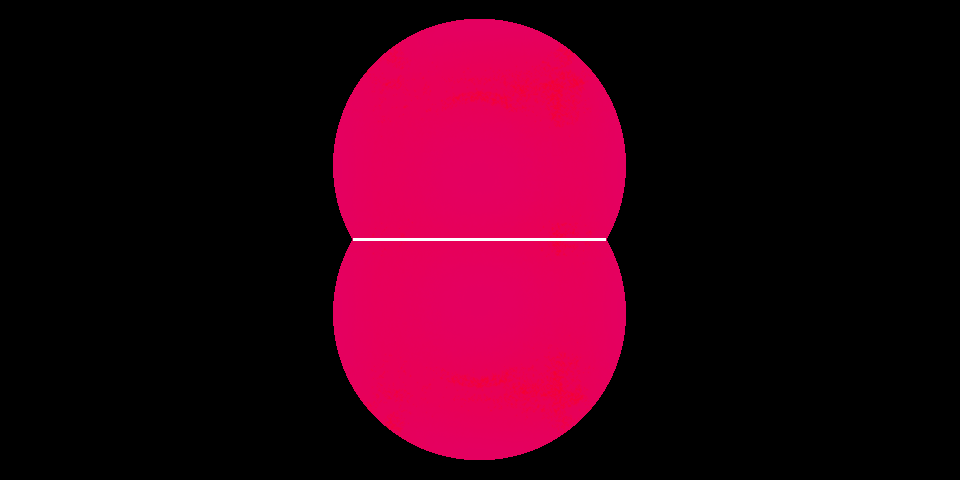
\includegraphics[height=1.5in]{images/union_sharp.png}
	\caption{Detected sharp edge on unioned spheres}
	\label{fig:UnionSharpEdge}
\end{figure}

$$
C=
\begin{bmatrix}
	{\partial N_x \over \partial x}&{\partial N_x \over \partial y}&{\partial N_x \over \partial z}\\
	{\partial N_y \over \partial x}&{\partial N_y \over \partial y}&{\partial N_y \over \partial z}\\
	{\partial N_z \over \partial x}&{\partial N_z \over \partial y}&{\partial N_z \over \partial z}
\end{bmatrix}
$$

To find the matrix C we still need the hessian matrix and normal vector
information; however, we do not need to calculate the gaussian and mean
curvatures.

$$
C_{ij} = {H_{ij} * ||\overrightarrow{G}|| - {G_i * dot_j \over
	||\overrightarrow{G}||} \over ||\overrightarrow{G}||^2}
$$\\\\\\\\
Using the non-zero eigenvalues of this matrix, we can find the $k1$ and $k2$
principal curvatures. If two eigenvalues are 0, then there is no curvature at
that point along either the tangent or bi-normal direction.

In a polygonizer, the curvature information can be used to determine how a
triangle should scale to accommodate the changes in the topology of the
underlying implicit surface. As the curvature approaches zero in absolute value,
the size of the triangle can grow, as it increases in absolute value, the size
of the triangle can shrink. The curvature can also be used to determine where
sharp edges occur, which will allow give the polygonizer more information about
what is happening at the given location where the normal vector may be wrong.

\subsection{Bounding Volume Hierarchies}
We implemented the bounding volume hierarchy (bvh) using axis-aligned bounding
boxes(AABB). We used this construction due to the simplicity and speed of the
intersection testing. From the use of AABB for rendering and collision
detection in video games, many optimized methods of intersection have been
developed\cite{Williams}. We implemented bvh to assist with speed of
evaluation, and convergence of the secant method for ray-tracing purposes.

\section{Findings}
In this section, we describe how the decisions made effected the resulting
speed and robustness of the blob tree.

\subsection{Scene Graph}

We performed the tests on the image shown in figure \ref{fig:Scenegraph}. The
scene is composed of four spheres. Two spheres are translated along the $y$
axis by $0.2$ and $-0.2$, then intersected creating the object $i1$. The other
two spheres are translated along the $x$ axis by $0.8$ and $-0.8$, and are
unioned creating the object $u1$. A final union operation joins both $i1$ and
$u1$, forming the object $u2$. $u2$ is then rendered.

\begin{table}[htbp]
	\centering
	\begin{tabular}{c | p{17pt} p{24pt} p{20pt} | p{17pt} p{24pt} p{20pt}}
No O3 & \multicolumn{3}{c |} {Instancing} & \multicolumn{3}{c } {No Instancing}\\
	& Time & Memory & Faults  & Time & Memory & Faults \\\hline
	& 22067 & 8228 & 836 & 22064 & 8476 & 819 \\
	& 22028 & 8280 & 838 & 22233 & 8356 & 762 \\
	& 22092 & 8316 & 834 & 22267 & 8456 & 901 \\
	& 22114 & 8316 & 836 & 22100 & 8492 & 903 \\
	& 22108 & 8224 & 1346& 22092 & 8416 & 900 \\\hline
mean	& 22081 & 8273 & 938 & 22151 & 8439 & 873 \\
std	& 35.15 & 45.2 & 228 & 91.97 & 54.51 & 62.07 \\\hline
O3 & \multicolumn{3}{c |} {Instancing} & \multicolumn{3}{c } {No Instancing}\\
	& Time & Memory & Faults  & Time & Memory & Faults \\\hline
	& 3238 & 8132 & 1250 & 3538 & 8336 & 1271 \\
	& 3232 & 8000 & 741 & 3507 & 8304 & 1270 \\
	& 3243 & 8152 & 743 & 3521 & 8408 & 759 \\
	& 3341 & 7964 & 739 & 3525 & 8504 & 760 \\
	& 3270 & 8032 & 1251 & 3555 & 8452 & 760 \\\hline
	mean & 3265 & 8056 & 944.8 & 3529 & 8401 & 964 \\
	std & 45.01 & 82.41 & 279.07 & 18.17 & 82.00 & 279.80\\\hline
	\end{tabular}
	\caption{Ray-trace statistics with scene graph}
	\label{tab:Scenegraph_performance}
\end{table}

We can see the effect of the scene graph and instancing in table
\ref{tab:Scenegraph_performance}.  We found that the implementation compiled
with no optimizations behaved quite differently than the implementation
compiled with optimizations.

With O3 optimizations applied, we found that the stability of the memory usage
decreased from the compilation with optimizations disabled, however memory
usage itself dropped. Furthermore optimizations improved the memory savings of
instancing.

For both compilations, the cpu time of the ray-tracer benefited from the
addition of instancing and a scene graph structure.

Page faults behaved a little differently though. The unoptimized compilation
with instancing suffered more page faults than the unoptimized compilation
without instancing. The optimizations seemed to create two bands of trial. One
band had elevated page faults over 1200 for the run, and the other band had
lower page faults in the 700's for a given run. Between instancing and no
instancing with optimization compilation, we noticed that the number of faults
decreased by roughly 20 with instancing and scene-graph construction.

\subsection{Bounding Volume Hierarchies}
We found that while the bvh greatly improved the rate of convergence of the
secant method, taking an average of four iterations with the bvh versus the
twenty iterations without, and increased the number of locations where it did
converge, we did not find that our naive approach had any effect on the overall
speed of the ray tracing program, which should have received the most benefit
from such a structure.

Furthermore, we were unable to get performance increase from using the bvh to
remove sections of the tree when evaluating the field value and computing
normal vectors.

\subsection{Limitations}
Our implementation of the implicit system only describes primitive spheres. No
tests have been done with other primitive shapes, and may not work. From
speculation, we believe that our implementation can be generalized for any
arbitrary primitive, so long as it can provide a method for calculating the
normal vector of a point. In the worst case, the normal value can be found
from sampling techniques\cite{Stam2011}.

\section{Future Work}
\subsection{BVH}
We would like to look into utilizing the bounding volume hierarchy to get more
performance from the system. While optimized methods were used for testing and
locating intersection points, we would like to use the bvh to determine when we
need to evaluate a branch of the subtree. It is evident that more work is
necessary to get the kind of performance boost we would like to see.

\subsection{Primitives}
Another area on extending the blob tree is implementing more primitive skeletal
objects, such as a: torus, cube, and line primitive. The implementation of the
normal calculation could remain the same, but the normal calculations for the
other primitives would either have to be sampled\cite{Stam2011} or specific
methods for the desired shape could be implemented. If the second approach is
taken, further testing would be required to ensure that the normal remains a
weighted linear combination of the normal vectors for a given point over the
component primitive objects.

\subsection{Field falloff functions}
As of this time, we have implemented and worked with the Geoff
function (\ref{eq:GeoffFunction}). Future work could include observing the effects
of other \fff s, or simply implementing more for extended functionality.

\subsection{Operations}
There are two remaining operations that have yet to be implemented: difference
operation and warp. The difference operation allows the removal of volume from
one object defined by another object.

The warp operation is a group of deformations. In particular Barr deformations,
such as \textit{twist}, \textit{taper}, and \textit{bend}.

\section{Conclusions}
The blob tree is a powerful way to build complex geometry from simpler
primitive geometries. We describe a method of implementing a blob tree with the
ability to provide information about normal data and curvature. To improve the
robustness and performance, we build the tree as a scene graph and describe a
simple method of implementing a bounding volume hierarchy.

Many of our decisions improved the performance of our blob tree implementation
from a straight-forward blob tree design. The features of the blob tree
implementation make it usable in a variety of situations, including ray-tracing
and provide more information for various polygonization methods, allowing
improved triangle meshes.


\bibliographystyle{acmsiggraph}
\bibliography{references}
\end{document}

